\SourceLeaf{319}
\begin{center}\resizebox{4.6cm}{!}{%
\begin{tikzpicture}[x=1pt,y=-1pt]
\path[use as bounding box] (0,0) rectangle (914,561);
\path[fill=black,draw=none,even odd rule]
(73,524) -- (73,525) -- (76,528) -- (90,528) -- (93,525) -- (92,523) -- (90,523) -- (89,522) -- (87,522) -- (86,523) -- (84,522) -- (77,522) -- cycle
(66,525) -- (62,522) -- (56,523) -- (56,528) -- (57,527) -- (61,528) -- (62,527) -- (64,527) -- cycle
(184,522) -- (184,524) -- (188,526) -- (194,526) -- (196,524) -- (196,522) -- (193,522) -- (192,521) -- (185,521) -- cycle
(156,523) -- (156,524) -- (158,526) -- (164,526) -- (165,527) -- (171,526) -- (173,524) -- (173,522) -- (172,521) -- (159,521) -- cycle
(132,525) -- (135,527) -- (139,527) -- (140,526) -- (145,526) -- (147,524) -- (147,523) -- (143,521) -- (137,521) -- (136,522) -- (134,522) -- (132,524) -- cycle
(104,524) -- (104,525) -- (108,528) -- (114,528) -- (115,527) -- (120,527) -- (121,526) -- (121,523) -- (120,522) -- (112,522) -- (110,521) -- cycle
(771,311) -- (769,309) -- (764,311) -- (757,317) -- (757,319) -- (758,320) -- (762,320) -- (765,317) -- (769,316) -- (770,315) -- cycle
(792,294) -- (791,293) -- (787,293) -- (785,294) -- (777,301) -- (777,303) -- (778,304) -- (781,304) -- (783,303) -- (786,300) -- (787,300) -- (792,295) -- cycle
(813,275) -- (812,274) -- (810,274) -- (803,278) -- (797,284) -- (797,286) -- (800,288) -- (805,286) -- (811,281) -- (811,280) -- (813,278) -- cycle
(835,258) -- (834,257) -- (830,257) -- (828,258) -- (819,266) -- (818,266) -- (817,268) -- (819,270) -- (823,270) -- (825,269) -- (835,260) -- cycle
(855,241) -- (850,240) -- (848,242) -- (847,242) -- (842,247) -- (842,250) -- (843,251) -- (847,251) -- (849,249) -- (850,249) -- (854,245) -- cycle
(875,225) -- (869,225) -- (867,226) -- (861,232) -- (861,233) -- (863,235) -- (869,233) -- (874,228) -- cycle
(755,327) -- (753,325) -- (744,325) -- (739,328) -- (728,329) -- (727,330) -- (727,332) -- (728,333) -- (732,333) -- (737,331) -- (739,333) -- (735,337) -- (734,337) -- (724,345) -- (721,346) -- (712,355) -- (711,355) -- (707,359) -- (703,361) -- (698,366) -- (693,369) -- (681,381) -- (680,381) -- (663,396) -- (658,399) -- (651,406) -- (646,409) -- (636,418) -- (633,419) -- (625,427) -- (624,427) -- (619,432) -- (618,432) -- (609,441) -- (607,441) -- (602,446) -- (597,449) -- (590,456) -- (585,459) -- (579,465) -- (578,465) -- (574,469) -- (569,472) -- (561,480) -- (560,480) -- (556,484) -- (553,485) -- (533,503) -- (532,503) -- (521,512) -- (519,512) -- (518,511) -- (518,508) -- (519,507) -- (519,503) -- (521,500) -- (521,494) -- (523,492) -- (523,485) -- (524,484) -- (524,480) -- (525,479) -- (526,474) -- (528,471) -- (528,462) -- (529,461) -- (529,456) -- (530,455) -- (530,452) -- (531,451) -- (532,438) -- (533,437) -- (532,434) -- (534,431) -- (534,427) -- (535,426) -- (535,419) -- (536,418) -- (536,415) -- (537,414) -- (537,409) -- (539,406) -- (539,398) -- (541,395) -- (542,384) -- (544,381) -- (544,374) -- (545,373) -- (545,369) -- (547,367) -- (547,363) -- (548,362) -- (547,357) -- (549,353) -- (549,348) -- (551,344) -- (553,329) -- (555,326) -- (554,320) -- (556,317) -- (556,309) -- (558,306) -- (558,304) -- (559,303) -- (559,299) -- (560,298) -- (560,291) -- (561,290) -- (560,289) -- (561,288) -- (560,287) -- (561,286) -- (561,282) -- (564,278) -- (563,276) -- (563,273) -- (564,272) -- (564,265) -- (565,264) -- (565,260) -- (566,259) -- (565,255) -- (568,251) -- (569,236) -- (571,234) -- (572,234) -- (573,235) -- (575,242) -- (578,244) -- (580,244) -- (582,242) -- (581,240) -- (581,237) -- (578,234) -- (577,230) -- (575,227) -- (574,218) -- (573,216) -- (571,214) -- (570,214) -- (566,218) -- (564,222) -- (560,226) -- (558,226) -- (549,236) -- (549,237) -- (551,239) -- (555,240) -- (557,239) -- (560,234) -- (563,231) -- (564,231) -- (566,233) -- (566,237) -- (564,240) -- (564,244) -- (563,245) -- (563,247) -- (560,251) -- (560,259) -- (558,261) -- (558,263) -- (557,264) -- (557,268) -- (556,269) -- (556,277) -- (555,278) -- (555,282) -- (554,283) -- (555,285) -- (555,288) -- (553,291) -- (553,296) -- (549,300) -- (551,302) -- (551,303) -- (548,306) -- (548,309) -- (550,311) -- (550,314) -- (549,315) -- (549,319) -- (548,320) -- (548,323) -- (547,324) -- (546,336) -- (545,337) -- (545,340) -- (544,341) -- (544,348) -- (543,349) -- (542,359) -- (541,360) -- (540,373) -- (539,374) -- (539,376) -- (537,378) -- (538,384) -- (536,387) -- (536,392) -- (535,393) -- (535,397) -- (534,398) -- (534,403) -- (533,404) -- (532,415) -- (531,416) -- (531,419) -- (530,420) -- (530,423) -- (529,424) -- (529,428) -- (528,429) -- (528,439) -- (527,440) -- (527,445) -- (526,446) -- (526,449) -- (525,450) -- (524,458) -- (521,463) -- (522,465) -- (522,468) -- (521,469) -- (521,476) -- (520,477) -- (520,481) -- (519,482) -- (519,485) -- (518,486) -- (517,501) -- (516,502) -- (516,506) -- (514,510) -- (514,516) -- (511,519) -- (501,519) -- (500,518) -- (498,518) -- (497,519) -- (489,519) -- (488,520) -- (483,520) -- (482,519) -- (472,519) -- (471,518) -- (469,518) -- (468,519) -- (464,519) -- (463,520) -- (453,520) -- (452,519) -- (448,519) -- (447,520) -- (437,520) -- (436,519) -- (430,519) -- (429,520) -- (427,519) -- (424,519) -- (423,520) -- (396,520) -- (395,519) -- (392,519) -- (391,520) -- (318,520) -- (317,521) -- (315,521) -- (314,520) -- (312,520) -- (311,521) -- (291,521) -- (290,520) -- (288,520) -- (287,521) -- (281,521) -- (280,520) -- (278,521) -- (271,521) -- (270,520) -- (267,520) -- (265,521) -- (264,520) -- (254,520) -- (253,521) -- (234,521) -- (233,522) -- (227,522) -- (224,519) -- (231,512) -- (230,510) -- (220,517) -- (217,517) -- (214,519) -- (212,519) -- (207,522) -- (207,524) -- (209,526) -- (211,527) -- (214,527) -- (216,529) -- (221,531) -- (224,534) -- (226,534) -- (227,533) -- (227,531) -- (224,528) -- (224,526) -- (225,525) -- (242,525) -- (243,526) -- (247,526) -- (248,525) -- (252,525) -- (253,526) -- (255,526) -- (256,525) -- (261,525) -- (262,526) -- (267,526) -- (268,525) -- (271,525) -- (272,526) -- (274,526) -- (275,525) -- (277,525) -- (278,526) -- (284,526) -- (285,525) -- (292,525) -- (293,526) -- (296,526) -- (297,525) -- (301,525) -- (302,526) -- (303,525) -- (328,525) -- (329,526) -- (331,525) -- (355,525) -- (357,526) -- (358,525) -- (376,525) -- (377,524) -- (385,524) -- (386,525) -- (388,525) -- (389,524) -- (407,525) -- (408,524) -- (417,524) -- (418,523) -- (420,523) -- (421,524) -- (438,524) -- (439,523) -- (441,523) -- (442,524) -- (453,524) -- (454,523) -- (460,523) -- (462,525) -- (464,524) -- (475,524) -- (476,523) -- (481,523) -- (482,524) -- (486,524) -- (487,523) -- (489,524) -- (502,524) -- (503,523) -- (505,524) -- (514,524) -- (516,523) -- (527,511) -- (533,508) -- (552,491) -- (554,491) -- (563,483) -- (566,482) -- (574,474) -- (576,474) -- (581,469) -- (586,466) -- (588,464) -- (588,463) -- (595,457) -- (597,457) -- (599,455) -- (603,453) -- (613,443) -- (616,442) -- (617,440) -- (629,429) -- (632,428) -- (639,421) -- (644,419) -- (650,413) -- (651,413) -- (662,403) -- (663,403) -- (684,383) -- (692,378) -- (697,373) -- (700,372) -- (710,362) -- (720,356) -- (724,351) -- (728,349) -- (732,344) -- (733,344) -- (737,340) -- (738,340) -- (743,335) -- (745,336) -- (745,338) -- (744,339) -- (744,342) -- (742,346) -- (742,350) -- (743,351) -- (745,351) -- (747,349) -- (747,345) -- (748,344) -- (749,338) -- (752,334) -- (752,332) -- (755,329) -- cycle
(579,171) -- (577,171) -- (575,173) -- (574,175) -- (574,180) -- (572,184) -- (572,193) -- (569,199) -- (569,202) -- (572,205) -- (574,205) -- (576,202) -- (577,191) -- (579,188) -- (579,185) -- (580,184) -- (580,180) -- (579,178) -- (581,175) -- (581,173) -- cycle
(583,142) -- (581,143) -- (581,145) -- (579,148) -- (579,152) -- (577,154) -- (577,158) -- (580,162) -- (581,162) -- (584,159) -- (584,155) -- (585,154) -- (585,151) -- (587,147) -- (587,145) -- cycle
(589,114) -- (587,114) -- (584,117) -- (585,120) -- (583,124) -- (583,128) -- (585,130) -- (588,130) -- (589,129) -- (589,126) -- (591,123) -- (591,116) -- cycle
(595,86) -- (592,86) -- (590,88) -- (590,91) -- (588,94) -- (588,98) -- (586,100) -- (586,101) -- (589,104) -- (592,104) -- (595,101) -- (595,98) -- (596,97) -- (596,92) -- (597,91) -- (596,87) -- cycle
(599,61) -- (597,61) -- (594,65) -- (594,68) -- (592,71) -- (592,74) -- (594,76) -- (598,76) -- (600,73) -- (600,66) -- (601,65) -- (601,63) -- cycle;
\node[inner sep=0pt,font=\fontsize{10}{10}\selectfont] at (599.5,29.5) {\scalebox{5.841}{$B$}};
\node[inner sep=0pt,font=\fontsize{10}{10}\selectfont] at (887.0,201.5) {\scalebox{5.841}{$A$}};
\node[inner sep=0pt,font=\fontsize{10}{10}\selectfont] at (28.0,526.0) {\scalebox{6.138}{$C$}};
\node[inner sep=0pt,font=\fontsize{10}{10}\selectfont] at (564.5,528.0) {\scalebox{6.534}{$X$}};
\end{tikzpicture}%
}
\hspace{.8cm}\resizebox{3.4cm}{!}{%
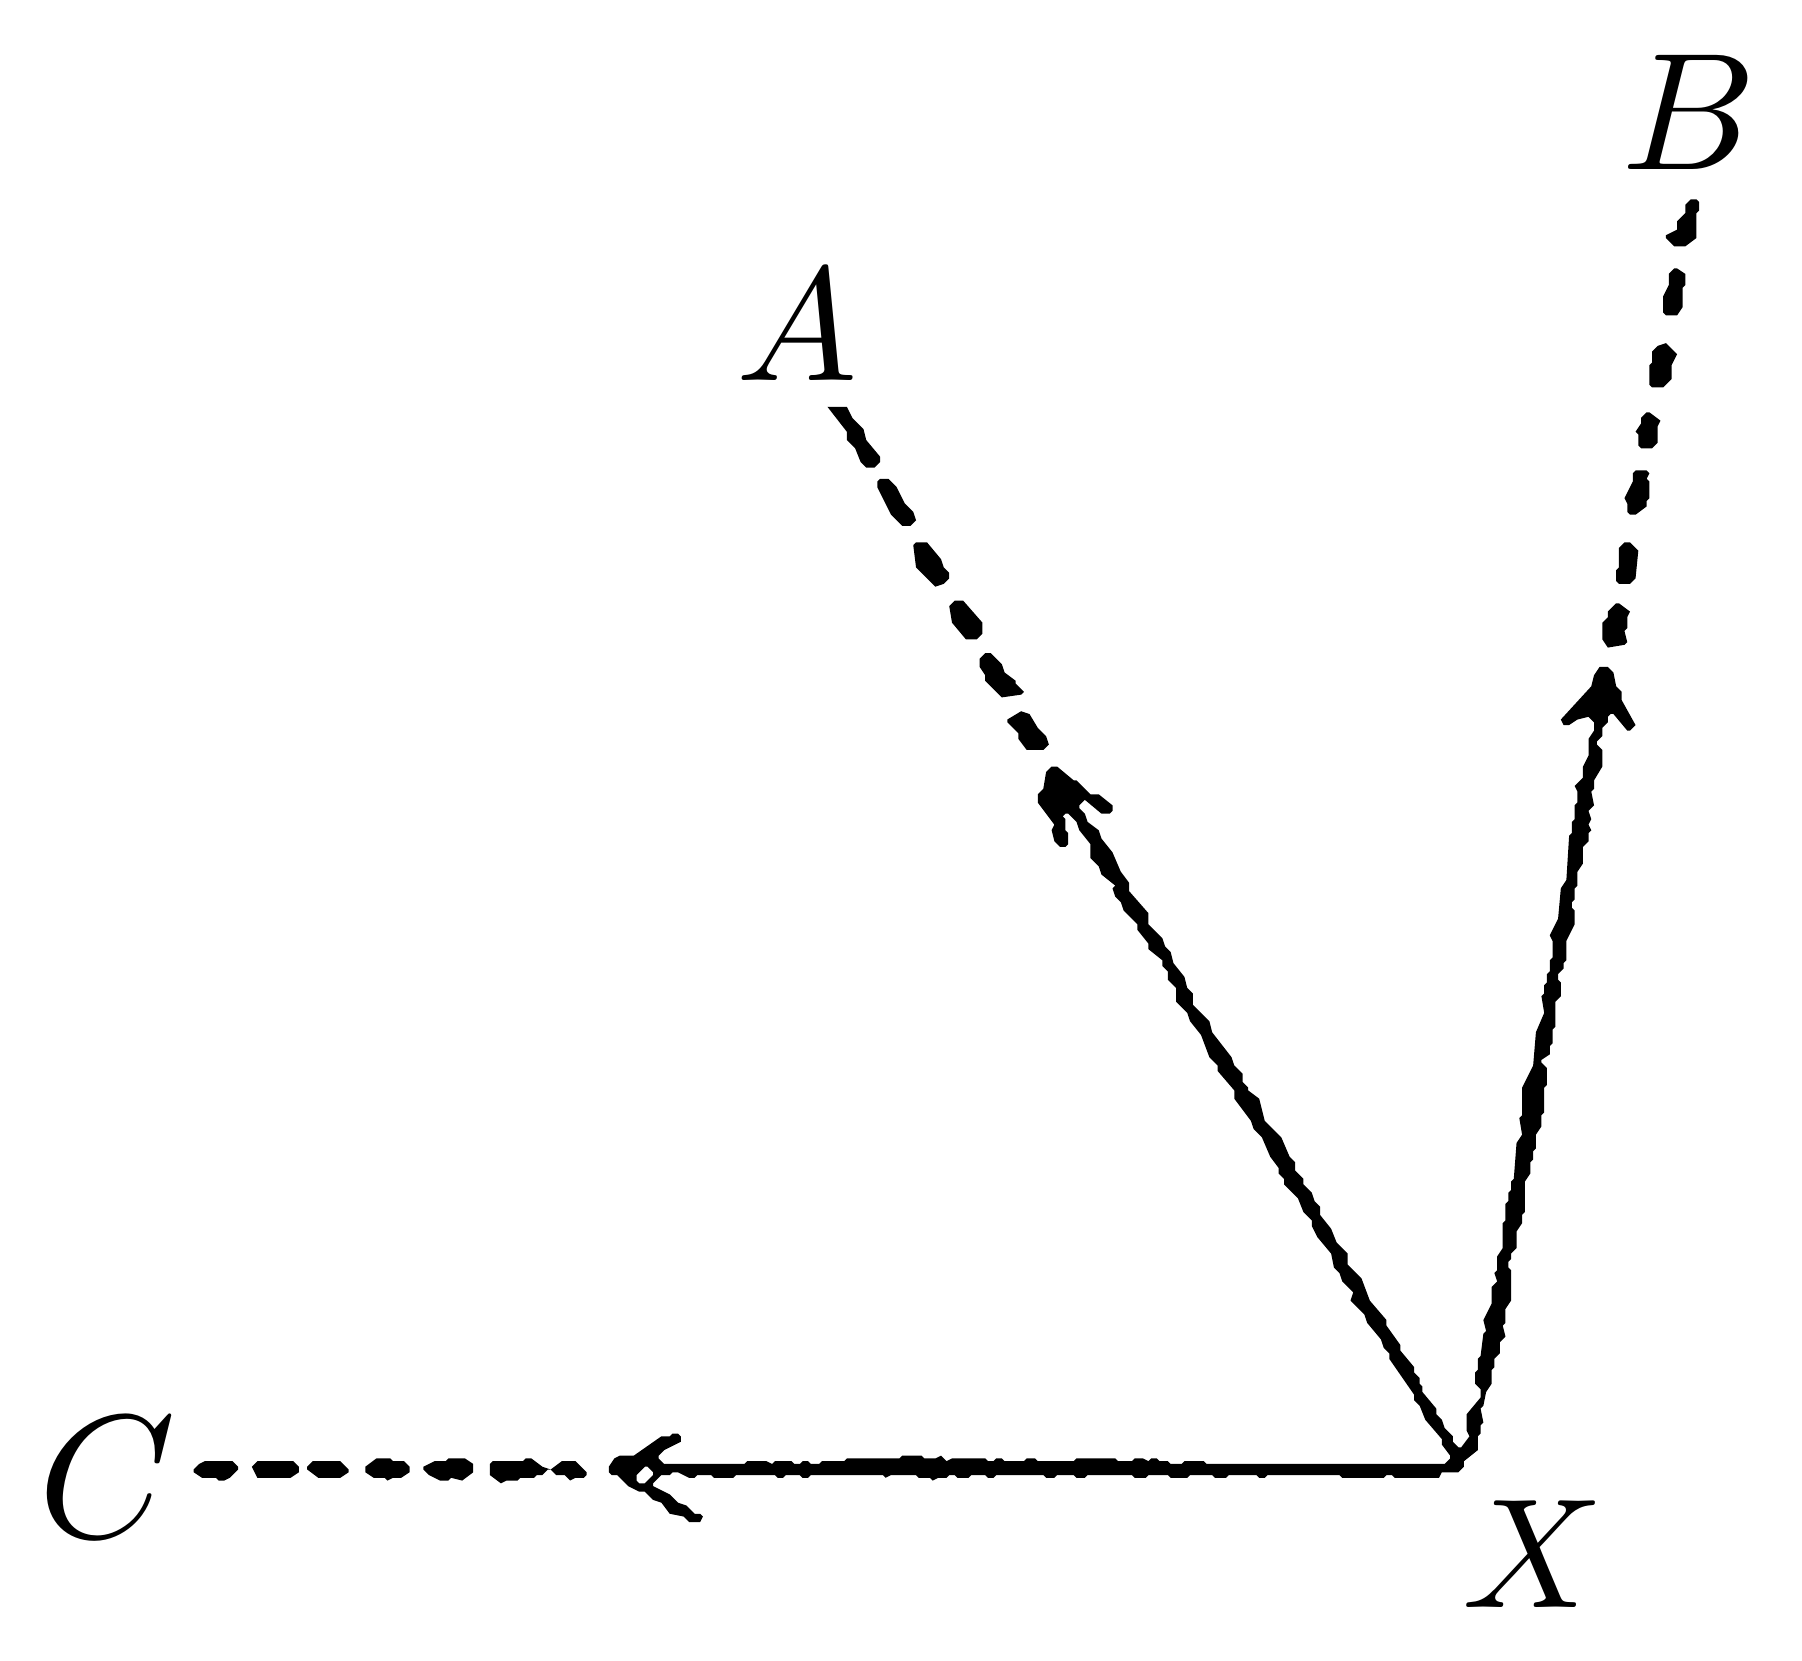
\begin{tikzpicture}[x=1pt,y=-1pt]
\path[use as bounding box] (0,0) rectangle (631,580);
\path[fill=black,draw=none,even odd rule]
(101,520) -- (101,521) -- (105,524) -- (113,524) -- (116,522) -- (116,521) -- (113,518) -- (103,518) -- cycle
(81,520) -- (83,524) -- (95,524) -- (98,522) -- (98,520) -- (96,518) -- (83,518) -- cycle
(60,522) -- (63,524) -- (68,524) -- (69,525) -- (71,525) -- (73,524) -- (76,521) -- (76,520) -- (74,518) -- (64,518) -- (62,519) -- (60,521) -- cycle
(167,519) -- (167,523) -- (171,526) -- (173,525) -- (177,525) -- (178,524) -- (183,524) -- (184,523) -- (186,523) -- (188,521) -- (189,521) -- (191,523) -- (194,523) -- (196,525) -- (198,524) -- (201,524) -- (202,523) -- (202,522) -- (198,518) -- (193,518) -- (189,521) -- (186,520) -- (182,517) -- (180,517) -- (179,518) -- (168,518) -- cycle
(143,520) -- (143,521) -- (145,523) -- (149,525) -- (152,525) -- (153,524) -- (157,525) -- (161,522) -- (161,519) -- (158,517) -- (152,517) -- (151,518) -- (147,518) -- cycle
(122,520) -- (122,522) -- (125,524) -- (129,524) -- (130,525) -- (132,524) -- (135,524) -- (138,522) -- (138,520) -- (136,518) -- (132,518) -- (131,517) -- (126,517) -- cycle
(354,250) -- (354,251) -- (358,255) -- (358,257) -- (361,261) -- (367,261) -- (369,259) -- (368,256) -- (365,253) -- (362,248) -- (359,247) -- cycle
(573,233) -- (571,231) -- (568,231) -- (566,234) -- (565,238) -- (554,250) -- (555,252) -- (557,252) -- (560,250) -- (564,249) -- (566,251) -- (566,254) -- (564,257) -- (564,263) -- (562,267) -- (562,271) -- (559,274) -- (560,276) -- (560,280) -- (559,281) -- (559,286) -- (558,287) -- (558,291) -- (557,292) -- (556,308) -- (554,311) -- (553,322) -- (550,328) -- (551,330) -- (551,336) -- (550,337) -- (550,341) -- (549,342) -- (549,345) -- (548,346) -- (548,349) -- (547,350) -- (548,356) -- (545,363) -- (544,375) -- (540,383) -- (540,393) -- (539,394) -- (540,400) -- (538,403) -- (537,416) -- (536,417) -- (536,420) -- (535,421) -- (535,424) -- (534,425) -- (534,431) -- (533,432) -- (533,441) -- (531,444) -- (531,449) -- (530,450) -- (531,453) -- (529,455) -- (529,461) -- (526,467) -- (527,471) -- (526,472) -- (525,480) -- (524,481) -- (524,485) -- (523,486) -- (523,490) -- (525,492) -- (525,495) -- (520,501) -- (520,507) -- (521,509) -- (518,513) -- (517,513) -- (515,511) -- (515,509) -- (512,506) -- (511,503) -- (509,501) -- (509,499) -- (504,493) -- (504,491) -- (503,490) -- (503,488) -- (501,486) -- (501,484) -- (496,478) -- (496,476) -- (491,469) -- (491,467) -- (485,460) -- (482,452) -- (477,447) -- (477,443) -- (473,439) -- (471,434) -- (467,429) -- (467,426) -- (465,424) -- (464,421) -- (461,418) -- (461,416) -- (458,413) -- (458,410) -- (456,408) -- (453,401) -- (447,395) -- (445,387) -- (441,384) -- (441,383) -- (439,381) -- (439,378) -- (436,375) -- (435,372) -- (428,363) -- (427,359) -- (421,353) -- (421,349) -- (419,347) -- (418,343) -- (414,338) -- (413,334) -- (411,332) -- (410,329) -- (405,324) -- (405,320) -- (398,312) -- (398,309) -- (395,305) -- (392,298) -- (388,293) -- (387,290) -- (383,287) -- (382,284) -- (380,282) -- (380,281) -- (382,279) -- (388,284) -- (391,284) -- (392,283) -- (392,281) -- (387,277) -- (384,277) -- (379,272) -- (378,272) -- (372,267) -- (370,267) -- (368,269) -- (367,275) -- (365,277) -- (365,280) -- (371,288) -- (370,290) -- (371,294) -- (373,296) -- (375,296) -- (376,295) -- (376,291) -- (375,290) -- (375,286) -- (374,285) -- (375,284) -- (376,284) -- (379,287) -- (380,290) -- (384,295) -- (384,300) -- (387,303) -- (388,306) -- (393,310) -- (392,311) -- (393,314) -- (395,316) -- (396,319) -- (401,324) -- (401,326) -- (405,331) -- (405,333) -- (410,337) -- (410,339) -- (412,341) -- (412,344) -- (415,347) -- (415,352) -- (419,356) -- (420,359) -- (424,364) -- (427,372) -- (430,375) -- (430,377) -- (436,384) -- (436,387) -- (442,395) -- (443,398) -- (446,401) -- (449,408) -- (452,412) -- (452,414) -- (454,416) -- (454,418) -- (459,423) -- (461,428) -- (464,431) -- (464,433) -- (466,437) -- (471,443) -- (472,448) -- (474,450) -- (475,453) -- (479,457) -- (478,460) -- (483,465) -- (484,468) -- (489,474) -- (490,477) -- (492,479) -- (492,481) -- (501,494) -- (501,496) -- (503,498) -- (505,503) -- (511,510) -- (511,512) -- (514,516) -- (514,517) -- (512,519) -- (426,519) -- (425,518) -- (418,518) -- (417,519) -- (413,519) -- (412,518) -- (409,518) -- (408,517) -- (406,517) -- (405,518) -- (403,517) -- (400,517) -- (399,518) -- (394,518) -- (393,517) -- (379,517) -- (378,518) -- (365,518) -- (364,517) -- (361,517) -- (360,518) -- (353,518) -- (352,517) -- (350,517) -- (349,518) -- (347,518) -- (346,517) -- (334,517) -- (332,518) -- (330,516) -- (328,517) -- (324,517) -- (323,516) -- (316,516) -- (315,517) -- (296,517) -- (295,518) -- (287,518) -- (286,519) -- (283,519) -- (282,518) -- (280,518) -- (279,519) -- (277,519) -- (276,518) -- (270,518) -- (269,519) -- (267,518) -- (260,518) -- (259,519) -- (230,519) -- (228,517) -- (228,516) -- (230,514) -- (236,511) -- (236,509) -- (235,508) -- (233,508) -- (232,509) -- (229,509) -- (219,516) -- (214,516) -- (212,517) -- (210,520) -- (210,522) -- (211,523) -- (213,523) -- (217,527) -- (221,529) -- (223,529) -- (226,532) -- (229,533) -- (232,537) -- (237,538) -- (239,540) -- (243,540) -- (244,538) -- (243,537) -- (241,537) -- (238,534) -- (235,533) -- (232,530) -- (226,527) -- (226,526) -- (229,523) -- (232,523) -- (233,522) -- (235,522) -- (239,524) -- (241,524) -- (242,523) -- (247,523) -- (248,524) -- (255,524) -- (256,523) -- (270,523) -- (271,524) -- (273,524) -- (274,523) -- (279,523) -- (280,524) -- (282,524) -- (283,523) -- (309,523) -- (310,524) -- (312,523) -- (321,523) -- (322,524) -- (326,524) -- (327,525) -- (329,524) -- (332,524) -- (333,523) -- (335,523) -- (336,524) -- (340,524) -- (341,523) -- (346,523) -- (347,524) -- (349,524) -- (350,523) -- (367,523) -- (368,524) -- (371,524) -- (372,523) -- (378,523) -- (379,524) -- (382,524) -- (383,523) -- (399,523) -- (400,524) -- (404,524) -- (405,523) -- (412,523) -- (413,524) -- (419,524) -- (420,523) -- (428,523) -- (429,524) -- (433,524) -- (434,523) -- (444,523) -- (445,524) -- (447,524) -- (448,523) -- (474,523) -- (475,524) -- (490,524) -- (491,523) -- (493,523) -- (494,524) -- (510,524) -- (511,522) -- (517,522) -- (519,520) -- (519,518) -- (524,514) -- (524,509) -- (525,508) -- (525,505) -- (526,504) -- (525,499) -- (526,498) -- (527,493) -- (529,490) -- (529,485) -- (530,484) -- (530,481) -- (532,479) -- (532,475) -- (534,473) -- (533,469) -- (534,468) -- (534,463) -- (536,460) -- (536,449) -- (535,448) -- (535,446) -- (536,445) -- (536,443) -- (538,441) -- (538,435) -- (540,432) -- (540,429) -- (541,428) -- (541,417) -- (543,414) -- (543,410) -- (544,409) -- (544,406) -- (545,405) -- (545,400) -- (547,397) -- (547,393) -- (548,392) -- (548,383) -- (549,382) -- (549,376) -- (547,374) -- (547,373) -- (550,371) -- (550,368) -- (551,367) -- (551,362) -- (552,361) -- (552,352) -- (554,350) -- (554,345) -- (553,344) -- (553,342) -- (555,340) -- (555,338) -- (556,337) -- (556,330) -- (559,324) -- (559,319) -- (558,318) -- (558,316) -- (559,315) -- (559,311) -- (560,310) -- (560,305) -- (562,302) -- (562,296) -- (564,294) -- (564,291) -- (565,290) -- (564,288) -- (565,286) -- (564,283) -- (566,281) -- (565,276) -- (566,275) -- (566,272) -- (569,267) -- (569,261) -- (567,259) -- (567,258) -- (569,256) -- (569,253) -- (571,251) -- (571,249) -- (572,248) -- (573,248) -- (578,254) -- (579,254) -- (581,252) -- (576,243) -- (576,240) -- (574,238) -- cycle
(224,520) -- (226,522) -- (226,523) -- (223,526) -- (221,526) -- (220,525) -- (220,523) -- (223,520) -- cycle
(346,226) -- (344,228) -- (344,231) -- (346,234) -- (346,236) -- (352,242) -- (359,241) -- (360,240) -- (357,237) -- (357,236) -- (353,233) -- (352,230) -- (348,226) -- cycle
(575,208) -- (574,208) -- (571,211) -- (571,213) -- (569,215) -- (569,221) -- (571,224) -- (577,223) -- (578,222) -- (577,218) -- (578,217) -- (578,213) -- (579,211) -- cycle
(335,207) -- (333,209) -- (334,215) -- (339,221) -- (343,221) -- (345,219) -- (345,215) -- (338,207) -- cycle
(579,186) -- (577,186) -- (575,188) -- (575,195) -- (574,196) -- (574,200) -- (575,201) -- (579,201) -- (581,199) -- (582,189) -- cycle
(321,186) -- (320,187) -- (321,195) -- (328,202) -- (331,201) -- (333,199) -- (333,197) -- (331,195) -- (330,192) -- (325,186) -- cycle
(308,163) -- (307,164) -- (307,166) -- (312,176) -- (316,180) -- (319,180) -- (321,178) -- (320,175) -- (317,172) -- (314,166) -- (311,163) -- cycle
(585,160) -- (581,160) -- (580,161) -- (580,164) -- (577,170) -- (578,172) -- (578,175) -- (579,176) -- (581,176) -- (585,173) -- (585,171) -- (586,170) -- (586,164) -- (585,163) -- (586,161) -- cycle
(586,139) -- (585,139) -- (583,141) -- (583,143) -- (581,146) -- (582,147) -- (582,151) -- (583,152) -- (587,152) -- (589,150) -- (589,144) -- (590,142) -- cycle
(289,137) -- (296,146) -- (296,149) -- (299,152) -- (301,157) -- (303,159) -- (306,159) -- (308,157) -- (308,155) -- (303,149) -- (302,145) -- (298,141) -- (296,137) -- cycle
(592,114) -- (589,115) -- (587,117) -- (587,121) -- (586,122) -- (586,129) -- (587,130) -- (591,130) -- (594,127) -- (594,122) -- (596,118) -- cycle
(596,87) -- (595,87) -- (593,89) -- (593,93) -- (591,97) -- (591,103) -- (592,104) -- (596,104) -- (598,101) -- (598,94) -- (599,93) -- (599,89) -- cycle
(603,62) -- (601,62) -- (599,64) -- (599,67) -- (596,70) -- (596,73) -- (592,75) -- (592,76) -- (595,79) -- (599,79) -- (603,76) -- (603,67) -- (604,66) -- (604,63) -- cycle;
\node[inner sep=0pt,font=\fontsize{10}{10}\selectfont] at (600.5,30.5) {\scalebox{6.039}{$B$}};
\node[inner sep=0pt,font=\fontsize{10}{10}\selectfont] at (278.0,107.5) {\scalebox{5.841}{$A$}};
\node[inner sep=0pt,font=\fontsize{10}{10}\selectfont] at (29.0,524.0) {\scalebox{6.336}{$C$}};
\node[inner sep=0pt,font=\fontsize{10}{10}\selectfont] at (544.0,551.5) {\scalebox{5.643}{$X$}};
\end{tikzpicture}%
}
\end{center}

die Fälle nicht gehörig unterschieden würden, oder, mit andern Worten, weil
man sonst nicht Ein Problem, sondern auf einmal vier verschiedene aufgeben
würde.

\textls[120]{Diess wohlverstanden}, sind nun alle bisherigen Behandlungen des Problems in
so fern unvollständig, als sie keine allgemeine Regel angeben, wonach man
vorgegebenen Datis gleich ansehen kann, ob sie zusammen bestehen können oder
nicht. Auch ohne bloss vom theoretischen Standpunkt auszugehen, scheint eine
Ergänzung dieses Mangels praktisch wünschenswerth, weil ja Data, die sich auf
einen wirklichen Fall in concreto beziehen sollen, wenn auch nicht durch
Neckerei, doch durch grobe Schreibfehler und Irrthum entstellt sein können,
deren Dasein sogleich in vielen Fällen erkennen zu können, doch auch dem
blossen Praktiker werth sein muss.

Allgemeine Regel verstehe ich so, dass man nicht für jeden speciellen Fall
eine eigene rohe Zeichnung machen soll. Denn wenn man das thun will, so wird
es jedesmal eben nicht schwer sein, über Möglichkeit oder Unmöglichkeit zu
urtheilen.

Das eben wird aber verlangt, dass Alle Fälle in Einer allgemeinen Regel
befasst werden sollen.

Sie schienen zu glauben, dass solche physische Unmöglichkeit oder
Unvereinbarkeit eben nur einzelne, vielleicht seltene, Fälle trifft, das ist
aber nicht so, sondern (abstrahirt von einer gewussten richtigen Beziehung
auf einen wirklichen Fall in concreto) gibt es dreimal so viel unmögliche als
mögliche Combinationen.

Das eben ist nun in dem allgemeinen Satz enthalten, welcher auf dem Zettel
steht. Nemlich:

\begin{quote}»Wenn die vorgeschriebenen Data möglich sind, so werden sie durch Abänderung
einer der drei Richtungen ($XA$, $XB$, $XC$) in die entgegengesetzte (um
$180^0$ verschieden) sogleich unmöglich«.\end{quote}
